
\chapter{Rotational Invariant Expansion\label{chpt:rotational-invariant-expansion}}

If a function $F(\mathbf{X_{1}},\mathbf{X_{2}})$, $\mathbf{X_{i}}\equiv(\mathbf{r_{i}},\mathbf{\Omega_{i}})$
has transitional and rotational invariance \citep{Blum_I}, it can
be expanded as
\begin{equation}
F(\mathbf{X_{1}},\mathbf{X_{2}})=\sum_{mnl\mu\nu}F_{\mu\nu}^{mnl}(\left\Vert \mathbf{r_{12}}\right\Vert )\Phi_{\mu\nu}^{mnl}(\mathbf{\Omega_{1}},\mathbf{\Omega_{2}},\mathbf{\hat{r_{12}}})\label{eq:pdf_on_rot_invar}
\end{equation}
where $\mathbf{r_{12}}\equiv\mathbf{r_{1}}-\mathbf{r_{2}}$ according
to the transitional invariance, and
\begin{equation}
\Phi_{\mu\nu}^{mnl}(\mathbf{\Omega_{1}},\mathbf{\Omega_{2}},\mathbf{\hat{r_{12}}})=f^{mnl}\sum_{\mu'\nu'\lambda'}\left(\begin{array}{ccc}
m & n & l\\
\mu' & \nu' & \lambda'
\end{array}\right)R_{\mu'\mu}^{m}(\mathbf{\Omega_{1}})R_{\nu'\nu}^{n}(\mathbf{\Omega_{2}})R_{\lambda'0}^{l}(\mathbf{\hat{r_{12}}})\label{eq:definition_rot_invar}
\end{equation}
where $R_{\mu'\mu}^{m}$ is the Wigner generalized spherical harmonics
or Wigner D-symbol defined in the same convention as Messiah \citep{Messiah}
(different than Edmonds \citep{Edmonds}). $f^{mnl}$ can be any arbitrary
non-zero constant \citep{Fries_Patey_1985}. Here we define $f^{mnl}=f^{m}f^{n}=\sqrt{2m+1}\sqrt{2n+1}$
according to the definition of Belloni \citep{Luc_2014}.

Two special cases are adopted in this thesis, these being the laboratory
coordinate system with particle 1 at origin (fixed frame) and intermolecular
coordinate system (local frame) shown in figure \ref{fig:coordinate_systems}.
Their formalism and symmetry properties are presented later.


\section{Orthogonality of $\Phi$}

The rotational invariant $\Phi$ in eq. (\ref{eq:definition_rot_invar})
is orthogonal, as proven below:
\begin{eqnarray}
\left\langle \Phi\mid\Phi_{2}\right\rangle  & = & \int\mathrm{d}\mathbf{\Omega_{1}}\mathrm{d}\mathbf{\Omega_{2}}\mathrm{d}\hat{\mathbf{r}}\Phi_{\mu\nu}^{mnl}(\mathbf{\Omega_{1}},\mathbf{\Omega_{2}},\mathbf{\hat{r_{12}}})\Phi_{\mu_{2}\nu_{2}}^{m_{2}n_{2}l_{2}*}(\mathbf{\Omega_{1}},\mathbf{\Omega_{2}},\mathbf{\hat{r_{12}}})\nonumber \\
 & = & f^{m}f^{n}f^{m_{2}}f^{n_{2}}\sum_{\mu'\nu'\lambda'}\left(\begin{array}{ccc}
m & n & l\\
\mu' & \nu' & \lambda'
\end{array}\right)\sum_{\mu_{2}'\nu_{2}'\lambda_{2}'}\left(\begin{array}{ccc}
m_{2} & n_{2} & l_{2}\\
\mu_{2}' & \nu_{2}' & \lambda_{2}'
\end{array}\right)\nonumber \\
 &  & \times\{\int\mathrm{d}\mathbf{\Omega_{1}}R_{\mu'\mu}^{m}(\mathbf{\Omega_{1}})R_{\mu_{2}'\mu_{2}}^{m_{2}*}(\mathbf{\Omega_{1}})\nonumber \\
 &  & \left[\int\mathrm{d}\mathbf{\Omega_{2}}R_{\nu'\nu}^{n}(\mathbf{\Omega_{2}})R_{\nu_{2}'\nu_{2}}^{n_{2}*}(\mathbf{\Omega_{2}})\left(\int\mathrm{d}\hat{\mathbf{r}}R_{\lambda'0}^{l}(\mathbf{\hat{r_{12}}})R_{\lambda_{2}'0}^{l_{2}*}(\mathbf{\hat{r_{12}}})\right)\right]\}\nonumber \\
 & = & f^{m}f^{n}f^{m_{2}}f^{n_{2}}\sum_{\mu'\nu'\lambda'}\left(\begin{array}{ccc}
m & n & l\\
\mu' & \nu' & \lambda'
\end{array}\right)\sum_{\mu_{2}'\nu_{2}'\lambda_{2}'}\left(\begin{array}{ccc}
m_{2} & n_{2} & l_{2}\\
\mu_{2}' & \nu_{2}' & \lambda_{2}'
\end{array}\right)\nonumber \\
 &  & \times\delta_{m,m_{2}}\delta_{n,n_{2}}\delta_{l,l_{2}}\delta_{\mu,\mu_{2}}\delta_{\nu,\nu_{2}}\delta_{\mu',\mu_{2}'}\delta_{\nu',\nu_{2}'}\delta_{\lambda',\lambda_{2}'}\nonumber \\
 & = & \left(2l+1\right)^{-1}\sum_{\mu'\nu'\lambda'}\left(\begin{array}{ccc}
m & n & l\\
\mu' & \nu' & \lambda'
\end{array}\right)\left(\begin{array}{ccc}
m & n & l\\
\mu' & \nu' & \lambda'
\end{array}\right)
\end{eqnarray}
and using the orthogonality of 3j-symbol \citep{Edmonds}
\begin{equation}
\sum_{l\lambda'}\left(2l+1\right)\left(\begin{array}{ccc}
m & n & l\\
\mu_{1}' & \nu_{1}' & \lambda'
\end{array}\right)\left(\begin{array}{ccc}
m & n & l\\
\mu_{2}' & \nu_{2}' & \lambda'
\end{array}\right)=\delta_{\mu_{1}'\mu_{2}'}\delta_{\nu_{1}'\nu_{2}'}
\end{equation}


\begin{equation}
\sum_{\mu'\nu'}\left(\begin{array}{ccc}
m & n & l\\
\mu' & \nu' & \lambda'
\end{array}\right)\left(\begin{array}{ccc}
m & n & l_{2}\\
\mu' & \nu' & \lambda_{2}'
\end{array}\right)=\left(2l+1\right)^{-1}\delta_{ll_{2}}\delta_{\lambda_{1}'\lambda_{2}'}
\end{equation}
it gives
\begin{equation}
\left\langle \Phi\mid\Phi_{2}\right\rangle =\left(2l+1\right)^{-1}
\end{equation}



\section{Rotational invariance of $\Phi$}

In any coordinate system, the value of $\Phi_{\mu\nu}^{mnl}$ remains
the same. Here is a demonstration with the fixed and local
frame mentioned above, described in figure \ref{fig:coordinate_systems}.

Let's use the definition in eq. (\ref{eq:definition_rot_invar}):
\begin{equation}
\Phi_{\mu\nu}^{mnl}(\boldsymbol{\omega_{1}},\boldsymbol{\omega_{2}},0)=f^{mnl}\sum_{\mu''\nu''\lambda''}\left(\begin{array}{ccc}
m & n & l\\
\mu'' & \nu'' & \lambda''
\end{array}\right)R_{\mu''\mu}^{m}(\boldsymbol{\omega_{1}})R_{\nu''\nu}^{n}(\boldsymbol{\omega_{2}})R_{\lambda''0}^{l}(0)
\end{equation}
\begin{equation}
\Phi_{\mu\nu}^{mnl}(0,\mathbf{\Omega},\mathbf{\hat{r}})=f^{mnl}\sum_{\mu'\nu'\lambda'}\left(\begin{array}{ccc}
m & n & l\\
\mu' & \nu' & \lambda'
\end{array}\right)R_{\mu'\mu}^{m}(0)R_{\nu'\nu}^{n}(\mathbf{\Omega})R_{\lambda'0}^{l}(\mathbf{\hat{r}})
\end{equation}


The spherical harmonics have property \citep{Edmonds,Messiah}
\begin{equation}
R_{\mu'\mu}^{m}(0)=\sum_{\mu''}R_{\mu'\mu''}^{m}(\mathbf{\hat{r}})R_{\mu''\mu}^{m}(\boldsymbol{\omega_{1}})
\end{equation}
\begin{equation}
R_{\nu'\nu}^{n}(\mathbf{\Omega})=\sum_{\nu''}R_{\nu'\nu''}^{n}(\mathbf{\hat{r}})R_{\nu''\nu}^{n}(\boldsymbol{\omega_{2}})
\end{equation}
\begin{equation}
R_{\lambda'0}^{l}(\mathbf{\hat{r}})=\sum_{\lambda''}R_{\lambda'\lambda''}^{l}(\mathbf{\hat{r}})R_{\lambda''0}^{l}(0)
\end{equation}
so
\begin{align}
\Phi_{\mu\nu}^{mnl}(0,\mathbf{\Omega},\mathbf{\hat{r}}) & =f^{mnl}\sum_{\mu''\nu''\lambda''}R_{\mu''\mu}^{m}(\boldsymbol{\omega_{1}})R_{\nu''\nu}^{n}(\boldsymbol{\omega_{2}})R_{\lambda''0}^{l}(0)\times\nonumber \\
 & \left[\sum_{\mu'\nu'\lambda'}\left(\begin{array}{ccc}
m & n & l\\
\mu' & \nu' & \lambda'
\end{array}\right)R_{\mu'\mu''}^{m}(\mathbf{\hat{r}})R_{\nu'\nu''}^{n}(\mathbf{\hat{r}})R_{\lambda'\lambda''}^{l}(\mathbf{\hat{r}})\right]
\end{align}


According to eq. (4.3.3) in Edmonds \citep{Edmonds} or (A.91) in
Gray & Gubbins \citep{Gray-Gubbins}
\begin{equation}
\sum_{\mu'\nu'\lambda'}\left(\begin{array}{ccc}
m & n & l\\
\mu' & \nu' & \lambda'
\end{array}\right)R_{\mu'\mu''}^{m*}(\mathbf{\hat{r}})R_{\nu'\nu''}^{n*}(\mathbf{\hat{r}})R_{\lambda'\lambda''}^{l*}(\mathbf{\hat{r}})=\left(\begin{array}{ccc}
m & n & l\\
\mu'' & \nu'' & \lambda''
\end{array}\right)
\end{equation}
where we can also prove
\begin{equation}
\sum_{\mu'\nu'\lambda'}\left(\begin{array}{ccc}
m & n & l\\
\mu' & \nu' & \lambda'
\end{array}\right)R_{\mu'\mu''}^{m}(\mathbf{\hat{r}})R_{\nu'\nu''}^{n}(\mathbf{\hat{r}})R_{\lambda'\lambda''}^{l}(\mathbf{\hat{r}})=\left(\begin{array}{ccc}
m & n & l\\
\mu'' & \nu'' & \lambda''
\end{array}\right)
\end{equation}
$\Phi_{\mu\nu}^{mnl}$ remains identical in the two cases
\begin{align}
\Phi_{\mu\nu}^{mnl}(0,\mathbf{\Omega},\mathbf{\hat{r}}) & =f^{mnl}\sum_{\mu''\nu''\lambda''}\left(\begin{array}{ccc}
m & n & l\\
\mu'' & \nu'' & \lambda''
\end{array}\right)R_{\mu''\mu}^{m}(\boldsymbol{\omega_{1}})R_{\nu''\nu}^{n}(\boldsymbol{\omega_{2}})R_{\lambda''0}^{l}(0)\nonumber \\
 & =\Phi_{\mu\nu}^{mnl}(\boldsymbol{\omega_{1}},\boldsymbol{\omega_{2}},0)
\end{align}


Therefore, the projection $F_{\mu\nu}^{mnl}(r)$ also remains rotational
invariant in these two coordinate systems.


\section{Transform in local frame}

In the intermolecular (local) coordinate system, the 2 molecules are
both positioned along the $z$ axis. Using the properties \citep{Edmonds,Gray-Gubbins,Messiah}
of generalized spherical harmonics:
\begin{equation}
\begin{array}{ccc}
R_{\mu'\mu}^{m}(\Theta,\Phi,\Psi)=\delta_{\mu'\mu} & \mathrm{if} & \Theta=\Phi=\Psi=0\end{array}
\end{equation}
 and 3j-symbol
\begin{eqnarray}
\left(\begin{array}{ccc}
m & n & l\\
\mu' & \nu' & \lambda'
\end{array}\right)\neq0 & \mathrm{only\,if} & \mu'+\nu'+\lambda'=0
\end{eqnarray}
 $\Phi_{\mu\nu}^{mnl}(\mathbf{\Omega_{1}},\mathbf{\Omega_{2}},\mathbf{\hat{r_{12}}})$
in eq. (\ref{eq:definition_rot_invar}) can be simplified to
\begin{equation}
\Phi_{\mu\nu}^{mnl}(\boldsymbol{\omega_{1}},\boldsymbol{\omega_{2}},0)=\sum_{\chi}\left(\begin{array}{ccc}
m & n & l\\
\chi & -\chi & 0
\end{array}\right)f^{m}f^{n}R_{\chi,\mu}^{m}(\boldsymbol{\omega_{1}})R_{-\chi,\nu}^{n}(\boldsymbol{\omega_{2}})\label{eq:phi_local}
\end{equation}


Thus eq. (\ref{eq:pdf_on_rot_invar}) becomes
\begin{eqnarray}
F(\boldsymbol{\omega_{1}},\boldsymbol{\omega_{2}},r) & = & \sum_{mnl\mu\nu}F_{\mu\nu}^{mnl}(r)\Phi_{\mu\nu}^{mnl}(\boldsymbol{\omega_{1}},\boldsymbol{\omega_{2}},0)\nonumber \\
 & = & \sum_{mnl\mu\nu}F_{\mu\nu}^{mnl}(r)f^{m}f^{n}\sum_{\chi}\left(\begin{array}{ccc}
m & n & l\\
\chi & -\chi & 0
\end{array}\right)R_{\chi\mu}^{m}(\boldsymbol{\omega_{1}})R_{-\chi\nu}^{n}(\boldsymbol{\omega_{2}})\label{eq:eq_total_local}
\end{eqnarray}
and the inverse equation
\begin{eqnarray}
F_{\mu\nu}^{mnl}(r) & = & \int\mathrm{d}\boldsymbol{\omega_{1}}\mathrm{d}\boldsymbol{\omega_{2}}F(\boldsymbol{\omega_{1}},\boldsymbol{\omega_{2}},r)\Phi_{\mu\nu}^{mnl*}(\boldsymbol{\omega_{1}},\boldsymbol{\omega_{2}},0)\nonumber \\
 & = & f^{m}f^{n}\sum_{\chi}\left(\begin{array}{ccc}
m & n & l\\
\chi & -\chi & 0
\end{array}\right)\times\nonumber \\
 &  & \int\mathrm{d}\boldsymbol{\omega_{1}}R_{\chi\mu}^{m*}(\boldsymbol{\omega_{1}})\int\mathrm{d}\boldsymbol{\omega_{2}}R_{-\chi\nu}^{n*}(\boldsymbol{\omega_{2}})F(\boldsymbol{\omega_{1}},\boldsymbol{\omega_{2}},r)
\end{eqnarray}


The function $F(\boldsymbol{\omega_{1}},\boldsymbol{\omega_{2}},r)$
and the projections $F_{\mu\nu}^{mnl}(r)$ can be transformed into each
other by 2 simple steps.


\subsection{Transform between $F_{\mu\nu}^{mnl}(r)$ and $F_{\mu\nu,\chi}^{mn}(r)$ }

Suppose
\begin{equation}
F_{\mu\nu,\chi}^{mn}(r)=\sum_{l}\left(\begin{array}{ccc}
m & n & l\\
\chi & -\chi & 0
\end{array}\right)F_{\mu\nu}^{mnl}(r)
\end{equation}


Using property of 3j-symbol \citep{Messiah}
\begin{equation}
\sum_{\chi}\left(\begin{array}{ccc}
m & n & l'\\
\chi & -\chi & 0
\end{array}\right)\left(\begin{array}{ccc}
m & n & l\\
\chi & -\chi & 0
\end{array}\right)=\frac{\delta_{l'l}}{2l+1}
\end{equation}
we have as the inverse transform

\begin{equation}
F_{\mu\nu}^{mnl}(r)=\left(2l+1\right)\sum_{\chi}\left(\begin{array}{ccc}
m & n & l\\
\chi & -\chi & 0
\end{array}\right)F_{\mu\nu,\chi}^{mn}(r)
\end{equation}


Thus Eq. (\ref{eq:eq_total_local}) becomes
\begin{eqnarray}
F(\boldsymbol{\omega_{1}},\boldsymbol{\omega_{2}},r) & = & \sum_{mnl\mu\nu}\left(2l+1\right)\sum_{\chi'}\left(\begin{array}{ccc}
m & n & l\\
\chi' & -\chi' & 0
\end{array}\right)F_{\mu\nu,\chi'}^{mn}(r)\times\nonumber \\
 &  & \sum_{\chi}\left(\begin{array}{ccc}
m & n & l\\
\chi & -\chi & 0
\end{array}\right)f^{m}f^{n}R_{\chi\mu}^{m}(\boldsymbol{\omega_{1}})R_{-\chi\nu}^{n}(\boldsymbol{\omega_{2}})\nonumber \\
 & = & \sum_{mn\mu\nu}\sum_{\chi'}\sum_{\chi}F_{\mu\nu,\chi'}^{mn}(r)f^{m}f^{n}R_{\chi\mu}^{m}(\boldsymbol{\omega_{1}})R_{-\chi\nu}^{n}(\boldsymbol{\omega_{2}})\times\nonumber \\
 &  & \sum_{l}\left(2l+1\right)\left(\begin{array}{ccc}
m & n & l\\
\chi' & -\chi' & 0
\end{array}\right)\left(\begin{array}{ccc}
m & n & l\\
\chi & -\chi & 0
\end{array}\right)
\end{eqnarray}


As
\begin{equation}
\sum_{l}\left(2l+1\right)\left(\begin{array}{ccc}
m & n & l\\
\chi' & -\chi' & 0
\end{array}\right)\left(\begin{array}{ccc}
m & n & l\\
\chi & -\chi & 0
\end{array}\right)=\delta_{\chi'\chi}
\end{equation}
we have
\begin{equation}
F(\boldsymbol{\omega_{1}},\boldsymbol{\omega_{2}},r)=\sum_{mn\mu\nu\chi}F_{\mu\nu,\chi}^{mn}(r)f^{m}f^{n}R_{\chi\mu}^{m}(\boldsymbol{\omega_{1}})R_{-\chi\nu}^{n}(\boldsymbol{\omega_{2}})\label{eq:local-forward}
\end{equation}
and
\begin{equation}
F_{\mu\nu,\chi}^{mn}(r)=\int\mathrm{d}\boldsymbol{\omega_{1}}\mathrm{d}\boldsymbol{\omega_{2}}F(\boldsymbol{\omega_{1}},\boldsymbol{\omega_{2}},r)f^{m}f^{n}R_{\chi\mu}^{m*}(\boldsymbol{\omega_{1}})R_{-\chi\nu}^{n*}(\boldsymbol{\omega_{2}})\label{eq:local_backward}
\end{equation}


Thus eq. (\ref{eq:local-forward}, \ref{eq:local_backward}) can be
performed either by fast generalized spherical harmonic transform
(FGSHT), or being developed into
\begin{equation}
F(\boldsymbol{\omega_{1}},\boldsymbol{\omega_{2}},r)=\sum_{mn\mu\nu\chi}F_{\mu\nu,\chi}^{mn}(r)f^{m}f^{n}r_{\chi\mu}^{m}(\theta_{1})r_{-\chi\nu}^{n}(\theta_{2})e^{-i\chi(\phi_{12}\equiv\phi_{1}-\phi_{2})}e^{-i\mu\psi_{1}}e^{-i\nu\psi_{2}}\label{eq:eq_s1_local}
\end{equation}
and transformed with FFT-3D.


\subsection{Rotational invariant transform with FFT-3D}

Suppose
\begin{equation}
F_{\mu\nu,\chi}^{m}(r,\theta_{2})=\sum_{n}F_{\mu\nu,\chi}^{mn}(r)f^{n}r_{-\chi\nu}^{n}(\theta_{2})
\end{equation}
then we have
\begin{equation}
F(\boldsymbol{\omega_{1}},\boldsymbol{\omega_{2}},r)=\sum_{m\mu\nu\chi}F_{\mu\nu,\chi}^{m}(r,\theta_{2})f^{m}r_{\chi\mu}^{m}(\theta_{1})e^{-i\chi\phi_{12}}e^{-i\mu\psi_{1}}e^{-i\nu\psi_{2}}
\end{equation}


The inverse transform should be
\begin{equation}
F_{\mu\nu,\chi}^{mn}(r)=\frac{1}{2}\int\mathrm{d}(\cos\theta_{2})F_{\mu\nu,\chi}^{m}(r,\theta_{2})r_{-\chi\nu}^{n}(\theta_{2})
\end{equation}


In the same way, suppose
\begin{equation}
F_{\mu\nu,\chi}(r,\theta_{1},\theta_{2})=\sum_{m}F_{\mu\nu,\chi}^{m}(r,\theta_{2})r_{\chi\mu}^{m}(\theta_{1})
\end{equation}
and the inverse transform
\begin{equation}
F_{\mu\nu,\chi}^{m}(r,\theta_{2})=\frac{1}{2}\int\mathrm{d}(\cos\theta_{1})F_{\mu\nu,\chi}(r,\theta_{1},\theta_{2})r_{\chi\mu}^{m}(\theta_{1})
\end{equation}


Then we have
\begin{equation}
F(r,\boldsymbol{\omega_{1}},\boldsymbol{\omega_{2}})=\sum_{\mu\nu\chi}F_{\mu\nu,\chi}(r,\theta_{1},\theta_{2})e^{-i\chi\phi_{12}}e^{-i\mu\psi_{1}}e^{-i\nu\psi_{2}}\label{eq:eq_s3_local}
\end{equation}
which can be treated as a normal FFT of 3 dimensions.


\section{Transform in fixed frame}

Similarly, in the laboratory coordinate system
\begin{equation}
\Phi_{\mu\nu}^{mnl}(0,\mathbf{\Omega},\mathbf{\hat{r}})=\sum_{\eta}\left(\begin{array}{ccc}
m & n & l\\
\mu & \eta & -\mu-\eta
\end{array}\right)f^{m}f^{n}R_{\eta,\nu}^{n}(\mathbf{\Omega})R_{-\mu-\eta,0}^{l}(\mathbf{\hat{r}})\label{eq:phi_global}
\end{equation}


The rotational invariant does not take advantage of the $\chi$ transform
as $\mu\neq0$. The expansion on rotational invariants should be calculated
directly.


\subsection{Expansion of $F(\mathbf{r},\mathbf{\Omega})$ on rotational invariants}

The total equation of the forward transform is as shown below:
\begin{equation}
F_{\mu\nu}^{mnl}(r)=f^{m}f^{n}\sum_{\eta}\left(\begin{array}{ccc}
m & n & l\\
\mu & \eta & -\mu-\eta
\end{array}\right)\int\mathrm{d}\hat{\mathbf{r}}R_{-\mu-\eta,0}^{l*}(\mathbf{\hat{r}})\int\mathrm{d}\mathbf{\Omega}F(r,\hat{\mathbf{r}},\mathbf{\Omega})R_{\eta,\nu}^{n*}(\mathbf{\Omega})
\end{equation}


Firstly, the FGSHT is performed.
\begin{equation}
F_{\eta\nu}^{n}(\mathbf{r})=\int\mathrm{d}\mathbf{\Omega}f^{n}F(\mathbf{r},\mathbf{\Omega})R_{\eta,\nu}^{n*}(\mathbf{\Omega})
\end{equation}


Then the spherical harmonic transform by histogram should give
\begin{equation}
F_{\eta\nu,\lambda}^{nl}(r)=\int\mathrm{d}\hat{\mathbf{r}}R_{\lambda0}^{l*}(\mathbf{\hat{r}})F_{\eta\nu}^{n}(r,\mathbf{\hat{r}})\label{eq:sht-1}
\end{equation}


As $F_{\eta\nu}^{n}(\mathbf{r})$ values are tabulated in the Cartesian
grid, we cannot use a quadrature approach without interpolation, so
the histogram approach is used.

Histogram for a function $f$ gives:

\begin{equation}
\overline{f}(r)=\int\mathrm{d}\theta_{r}\mathrm{d}\phi_{r}f(x,y,z)
\end{equation}
so if we want to compute

\begin{equation}
\overline{F}(r)=\int\mathrm{d}\theta_{r}\mathrm{d}\phi_{r}R_{\lambda0}^{l*}(x,y,z)F(x,y,z)
\end{equation}
we just need to propose 

\begin{equation}
f(x,y,z)=R_{\lambda0}^{l*}(x,y,z)F(x,y,z)
\end{equation}
For complex numbers $F_{\eta\nu}^{n}(\mathbf{r})$, the real and imagined
parts can be calculated separately.

The rotational matrices $R_{\lambda0}^{l*}(\mathbf{r})$ in Cartesian
coordinate systems can be pre-generated by recurrence as detailed in
appendix \ref{chpt:rotM-by-recurrence}. 

Finally, the combination of projections gives:
\begin{equation}
F_{\mu\nu}^{mnl}(r)=f^{m}\sum_{\eta}\left(\begin{array}{ccc}
m & n & l\\
\mu & \eta & -\mu-\eta
\end{array}\right)F_{\eta\nu,-\mu-\eta}^{nl}(r)
\end{equation}


\textcolor{red}{It should be noted that $F_{\mu\nu}^{mnl}(r)$ is
real?}


\subsection{Rebuild of $g(\mathbf{r},\mathbf{\Omega})$ from projections}

and the rebuild of $F(\mathbf{r},\mathbf{\Omega})$ in a certain orientation
is as simple as its definition
\begin{equation}
F(\mathbf{r},\mathbf{\Omega})=\sum_{mnl\mu\nu}F_{\mu\nu}^{mnl}(r)f^{m}f^{n}\sum_{\eta}\left(\begin{array}{ccc}
m & n & l\\
\mu & \eta & -\mu-\eta
\end{array}\right)R_{\eta\nu}^{n}(\mathbf{\Omega})R_{-\mu-\eta,0}^{l}(\mathbf{\hat{r}})\label{eq:bwd-1}
\end{equation}



\section{Symmetry}

In IEM and MDFT, the rotational invariant is used to describe the
solvent. It possess symmetric rules, introduced by the indistinguishability
of the two particles, symmetry properties of single particle, and its
real number property as a physical quantity. Here we list all the symmetric
rules concerning the 2-molecule system.


\subsection{Symmetric rules of $F(\boldsymbol{\omega_{1}},\boldsymbol{\omega_{2}})$
in intermolecular form}

\begin{figure}[h]
\begin{centering}
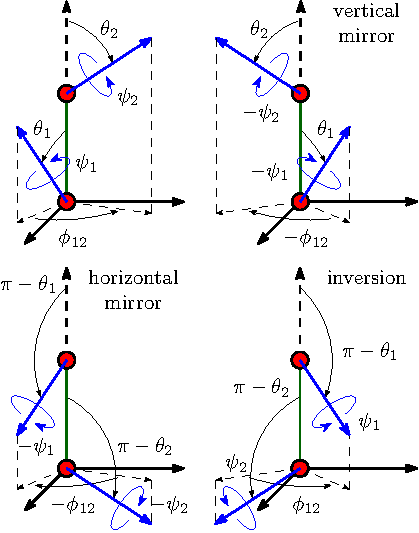
\includegraphics{_figure/symmetry_dcf}
\par\end{centering}

\caption{Symmetry operations of a 2-molecule system\label{fig:Symmetry-operations}}
\end{figure}


As shown in figure \ref{fig:Symmetry-operations}, function in intermolecular
coordinate system $F(\boldsymbol{\omega_{1}},\boldsymbol{\omega_{2}})\equiv F(\cos\theta_{1},\cos\theta_{2},\phi,\psi_{1},\psi_{2})$
possesses symmetry rules:
\begin{enumerate}
\item Symmetry of vertical mirror: 
\begin{equation}
F(\theta_{1},\theta_{2},\phi,\psi_{1},\psi_{2})=F(\theta_{1},\theta_{2},-\phi,-\psi_{1},-\psi_{2})
\end{equation}

\item Symmetry of inversion: 
\begin{equation}
F(\theta_{1},\theta_{2},\phi,\psi_{1},\psi_{2})=F(\pi-\theta_{2},\pi-\theta_{1},\phi,\psi_{2},\psi_{1})
\end{equation}

\end{enumerate}
And an additive symmetric rule is possessed by particles having 
\begin{enumerate}
\item \selectlanguage{english}%
[3.]\selectlanguage{american}%
Symmetry axe $\mathrm{C_{2n}}$: 
\begin{equation}
F(\theta_{1},\theta_{2},\phi,\psi_{1},\psi_{2})=F(\theta_{1},\theta_{2},\phi,\psi_{1}+\pi,\psi_{2}+\pi)
\end{equation}

\end{enumerate}

\subsection{Symmetric rules of rotational invariant projections}

\textcolor{red}{The definition of rotational invariant on $\chi$-transform
gives}

\textcolor{red}{
\begin{eqnarray*}
c(\theta_{1},\theta_{2},\phi_{12},\psi_{1},\psi_{2}) & = & \frac{1}{2l+1}\sum_{mn\mu\nu\chi}c_{\mu\nu,\chi}^{mn}(r)d_{\chi\mu}^{m}(\theta_{1})d_{\underline{\chi}\nu}^{n}(\theta_{2})e^{-i\chi\phi_{12}}e^{-i\mu\psi_{1}}e^{-i\nu\psi_{2}}
\end{eqnarray*}
}

\textcolor{red}{Thus}

\textcolor{red}{
\begin{eqnarray*}
c(\theta_{1},\theta_{2},-\phi_{12},-\psi_{1},-\psi_{2}) & = & \frac{1}{2l+1}\sum_{mn\mu\nu\chi}c_{\underline{\mu}\underline{\nu},\underline{\chi}}^{mn}(r)d_{\underline{\chi}\underline{\mu}}^{m}(\theta_{1})d_{\chi\underline{\nu}}^{n}(\theta_{2})e^{-i\chi\phi_{12}}e^{-i\mu\psi_{1}}e^{-i\nu\psi_{2}}\\
 & = & \frac{1}{2l+1}\sum_{mn\mu\nu\chi}\left(-\right)^{\mu+\nu}c_{\underline{\mu}\underline{\nu},\underline{\chi}}^{mn}(r)d_{\chi\mu}^{m}(\theta_{1})d_{\underline{\chi}\nu}^{n}(\theta_{2})e^{-i\chi\phi_{12}}e^{-i\mu\psi_{1}}e^{-i\nu\psi_{2}}
\end{eqnarray*}
\begin{eqnarray*}
c(\pi-\theta_{2},\pi-\theta_{1},\phi_{12},\psi_{2},\psi_{1}) & = & \frac{1}{2l+1}\sum_{mn\mu\nu\chi}c_{\mu\nu,\chi}^{mn}(r)d_{\chi\mu}^{m}(\pi-\theta_{2})d_{\underline{\chi}\nu}^{n}(\pi-\theta_{1})e^{-i\chi\phi_{12}}e^{-i\mu\psi_{2}}e^{-i\nu\psi_{1}}\\
 & = & \frac{1}{2l+1}\sum_{mn\mu\nu\chi}\left(-\right)^{m+n+\mu+\nu}c_{\nu\mu,\chi}^{nm}(r)d_{\chi\mu}^{m}(\theta_{1})d_{\underline{\chi}\nu}^{n}(\theta_{2})e^{-i\chi\phi_{12}}e^{-i\mu\psi_{1}}e^{-i\nu\psi_{2}}
\end{eqnarray*}
and $\mu$, $\nu$ are even.}

\textcolor{red}{Thus}

\textcolor{red}{
\[
c_{\mu\nu,\chi}^{mn}(r)=c_{\underline{\mu}\underline{\nu},\underline{\chi}}^{mn}(r)=\left(-\right)^{m+n}c_{\nu\mu,\chi}^{nm}(r)
\]
}

\textcolor{red}{(Need proof.)}

\textcolor{red}{
\[
\hat{c}_{\mu\nu,\underline{\chi}}^{mn}(\mathbf{k})=\left(-\right)^{m+n}\hat{c}_{\mu\nu,\chi}^{*mn}(\mathbf{k})
\]
}

\textcolor{red}{In MDFT, rotational invariant projections are used
to describe DCF. The original $c_{\mu\nu}^{mnl}(\mathbf{r})$ collected
by IEM is real.}
\begin{enumerate}
\item \textcolor{red}{With $r$ and $l$: As $c_{\mu\nu}^{mnl}(\mathbf{r})$
is real
\begin{equation}
F_{\underline{\mu}\underline{\nu}}^{mnl}(\mathbf{r})=\left(-\right)^{m+n+l}F_{\mu\nu}^{mnl}(\mathbf{r})
\end{equation}
As the two molecules are interchangeable, 
\begin{equation}
F_{\nu\mu}^{nml}(\mathbf{r})=\left(-\right)^{m+n}F_{\mu\nu}^{mnl}(\mathbf{r})
\end{equation}
}
\item \textcolor{red}{\selectlanguage{english}%
[2.]\selectlanguage{american}%
With $r$ and $\chi$:
\begin{equation}
F_{\mu\nu,\chi}^{mn}(\mathbf{r})=\sum_{\chi}\left(\begin{array}{ccc}
m & n & l\\
\chi & -\chi & 0
\end{array}\right)F_{\mu\nu}^{mnl}(\mathbf{r})
\end{equation}
\begin{equation}
F_{\underline{\mu}\underline{\nu},\underline{\chi}}^{mn}(\mathbf{r})=F_{\mu\nu,\chi}^{mn}(\mathbf{r})
\end{equation}
\begin{equation}
F_{\nu\mu,\chi}^{nm}(\mathbf{r})=\left(-\right)^{m+n}F_{\mu\nu,\chi}^{mn}(\mathbf{r})
\end{equation}
}
\item \textcolor{red}{\selectlanguage{english}%
[3.]\selectlanguage{american}%
With $k$ and $l$:
\begin{eqnarray}
\mathrm{TF}(c_{\mu\nu}^{mnl}(\mathbf{r})) & = & \hat{c}_{\mu\nu}^{mnl}(\mathbf{k})
\end{eqnarray}
 is real if $l$ is even, and is purely imaginary if $l$ is odd.}
\item \textcolor{red}{\selectlanguage{english}%
[4.]\selectlanguage{american}%
With $k$ and $\chi$:
\begin{equation}
F_{\mu\nu,\underline{\chi}}^{mn}(\mathbf{k})=\left(-\right)^{m+n}F_{\mu\nu,\chi}^{*mn}(\mathbf{k})
\end{equation}
}
\end{enumerate}
\textcolor{red}{Finally, if the solvent molecule possesses a symmetric
axe $\mathrm{C}_{2}$, $\mu$ and $\nu$ is even.} %I have a feeling 'symmetric axe' is not what you wanted to say here. Am I right?

\textcolor{red}{For spherical solutes, the $\mathbf{\Omega_{1}}$-dependence
vanishes so that $m=\mu=0$, only the terms $F_{0\nu}^{0nl}(r)$ is
not-zero.}
